\sloppy
\documentclass[14pt,a4paper,oneside]{extarticle}	% Размер основного шрифта и формата листа
\usepackage{xltxtra}						% Используется для вывода логотипа XeLaTeX
\usepackage{xunicode}						% Кодировка документа
\usepackage{polyglossia}					% Загружает пакет многоязыковой верстки
\newfontfamily\russianfont{Book Antiqua}
%\setmainfont{Liberation Serif}						% Основной шрифт текста
\setmainfont{Book Antiqua}
\setdefaultlanguage{russian}				% Основной язык текста
\setotherlanguage{english}					% Дополнительный язык текста
\linespread{1}							% Межстрочный интервал выбран полуторным
\usepackage[left=2.5cm,
right=1.5cm,vmargin=2.5cm]{geometry} % Отступы по краям листа
\bibliographystyle{ugost2008}

\usepackage{xcolor}
\usepackage{hyperref}
% Цвета для гиперссылок
\definecolor{linkcolor}{HTML}{359B08} % цвет ссылок
\definecolor{urlcolor}{HTML}{799B03} % цвет гиперссылок
\hypersetup{pdfstartview=FitH,  linkcolor=linkcolor,urlcolor=urlcolor, colorlinks=true}

%---------------------------%
%---- Пакеты расширений ----%
%---------------------------%
\usepackage{xcolor}
\usepackage{hyperref}
% Цвета для гиперссылок
\definecolor{linkcolor}{HTML}{359B08} % цвет ссылок
\definecolor{urlcolor}{HTML}{799B03} % цвет гиперссылок
\hypersetup{pdfstartview=FitH,  linkcolor=linkcolor,urlcolor=urlcolor, colorlinks=true}


\usepackage{verbatim,indentfirst}
\usepackage{cite,enumerate,float}
\usepackage{amsmath,amssymb,amsthm,amsfonts}

%---------------------------%
%--- Вставка иллюстраций ---%
%---------------------------%
\usepackage{graphicx}
\usepackage{subfigure}
%\graphicspath{{Images/}}
\usepackage{fontspec}

\begin{document}
%	\pagestyle{empty} %  выключаенм нумерацию
%\setcounter{page}{3}% Нумерация начинается с третьей страницы
%\renewcommand{\contentsname}{\center{Содержание}}
%\tableofcontents

\begin{center}
	%\addcontentsline{toc}{section}{Опыт 10. «Послушная» и  «непослушная» катушка}
	\subsection*{Свободные оси вращения}
\end{center}

\begin{figure}[H] 	% Окружение для вставки иллюстрации
	\centering 		% Выравнивание по центру
	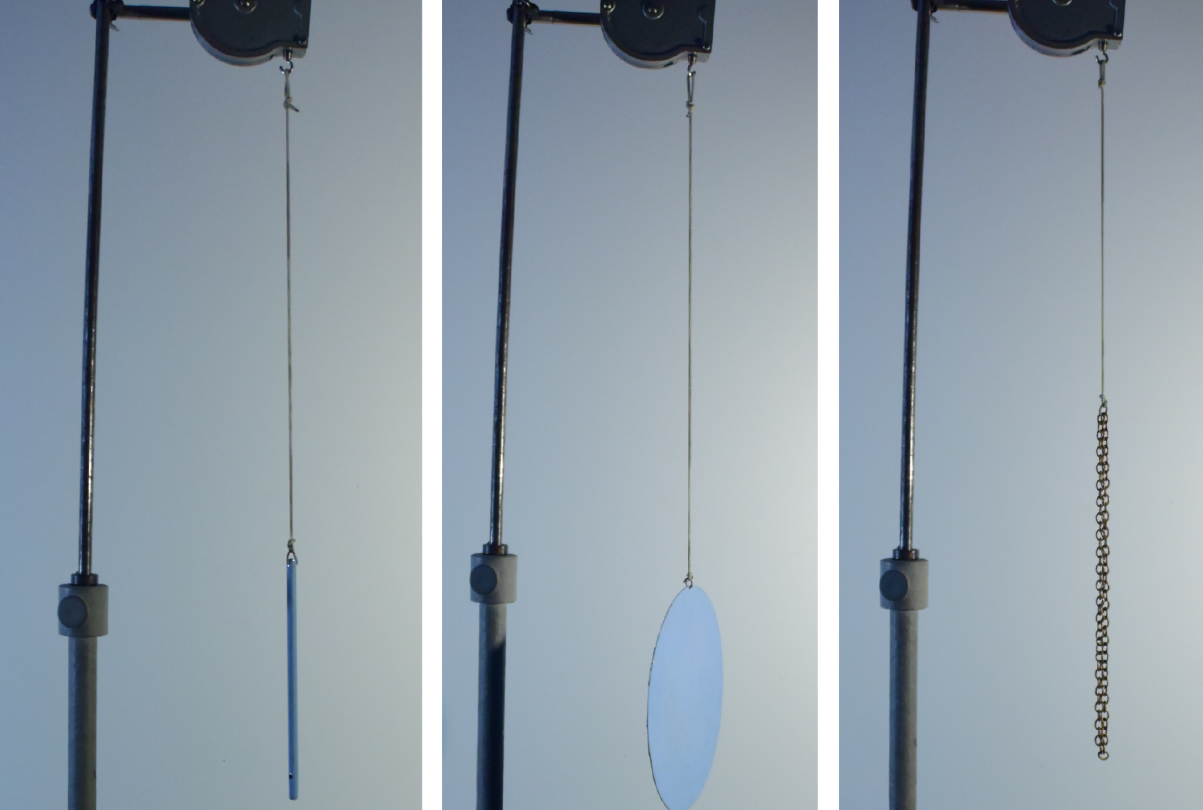
\includegraphics[width=0.9\linewidth]{freeaxis-1.png}
	\caption{Демонстрация устойчивости вращения тел вокруг свободных осей с наибольшим и наименьшим значениями момента инерции, и демонстрация того факта, что вращение с промежуточным моментом инерции неустойчиво}
	\label{freeaxis-1}
\end{figure}

\subsection*{\underline{Оборудование:}}

\begin{enumerate}
	\item Кусок поролона или пенопласта прямоугольной формы со сторонами различной длины (200:350:50 мм).
	\item Тела с подвесами (металлический диск, цилиндрический стержень, кольцо из цепочки).
	\item Червячная центробежная машина.
	\item Штатив.
\end{enumerate}

\newpage
\subsection*{\underline{Основные определения:}}

%Осевым М. и. тела относительно оси 
%z называется величина, определяемая равенством: 
%
%где mi — массы точек тела, hi — их расстояния от оси z, ? — массовая плотность, 
%V — объём тела. Величина Iz является мерой инертности тела при его вращении вокруг оси 
%(см. Вращательное движение ).

При вращении тела вокруг вала, концы которого закреплены, например, в подшипниках, на вал начинают действовать так называемые динамические силы реакции опоры.
Динамические реакции в отличие от статических действуют на движущееся тело.
Связанные с телом оси, при вращении относительно которых динамические реакции опор равны статическим, называются свободными осями. Другими словами, при вращении твердого тела относительно свободных осей вращения без трения внешние силы прикладывать ненужно.
При постоянной угловой скорости вращения динамические реакции перпендикулярны оси вращения (в отсутствие сил трения) и пропорциональны квадрату угловой скорости.

В любом теле произвольной формы существует три взаимно перпендикулярно оси, проходящие через центр масс тела, которые могут служить свободными осями вращения.
Их называют главными осями инерции.
Если взять тела одинаковой массы, но разной формы (диск, стержень или кольцо) и действовать на них равными моментами, то тела будут приобретать различные угловые ускорения. 
Их моменты инерции \textit{I} будут неодинаковыми, потому что у них разная форма.

\newpage
\subsection*{\underline{Краткое описание:}}

С цепочкой, стержнем и диском осуществляется демонстрация вращения тел около свободных осей с использованием имеющегося на центробежной машине крючка, к которому прикрепляются: а) стержень длиной 15-20 см и диаметром 1 см, б) металлический диск диаметром 12-20 см или в) цепочка в виде петли.

Подвешенная за один из концов металлический стержень при малых скоростях вращается в вертикальном положении, т.е. вокруг свободной оси с наибольшим моментом инерции (рис.\ref{freeaxis-2}).

\begin{figure}[H] 
	\centering 		
	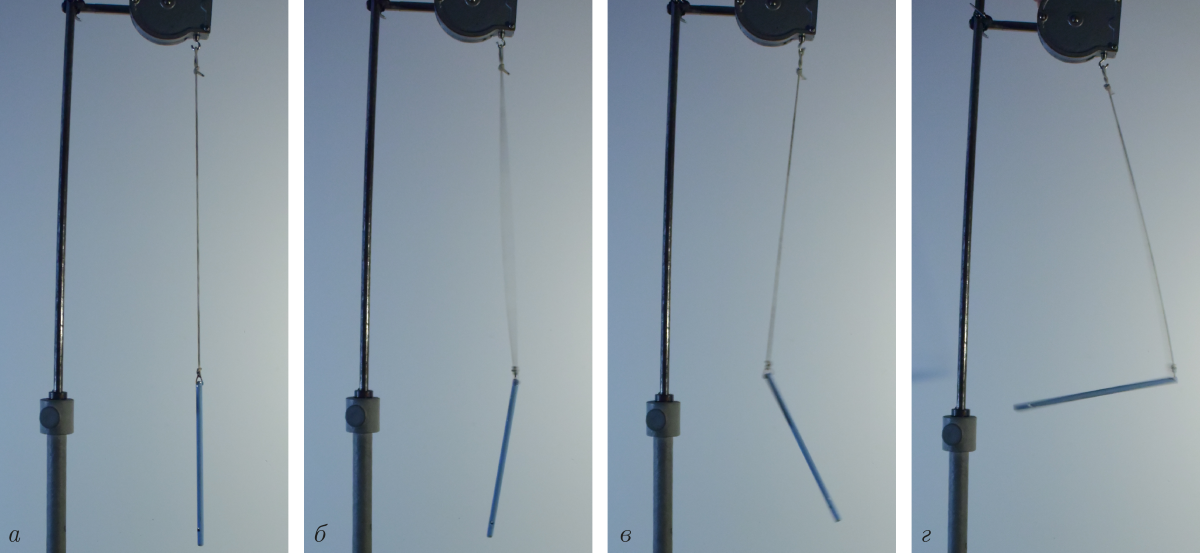
\includegraphics[width=0.9\linewidth]{freeaxis-2.png}
	\caption{Вращение цилиндрического стержня вокруг главной оси инерции}
	\label{freeaxis-2}
\end{figure}

При приведении машины во вращение стержень и диск, с увеличением угловой скорости, принимают горизонтальное положение (рис.\ref{freeaxis-3}), а цепочка, кроме того, растягивается в правильный круг (рис.\ref{freeaxis-4}).

Этот опыт демонстрирует вращение тел около свободных осей: при быстром вращении петля растягивается в круг, при чем ее плоскость располагается перпендикулярно к оси вращения. Центр круга цепочки будет лежать на продолжении оси вращения. Таким образом, цепочка будет устойчиво вращаться вокруг оси, проходящей через центр тяжести и перпендикулярной к плоскости образовавшегося кольца, т.е. вокруг оси с наибольшим моментом инерции.

\begin{figure}[H] 	
	\centering 		
	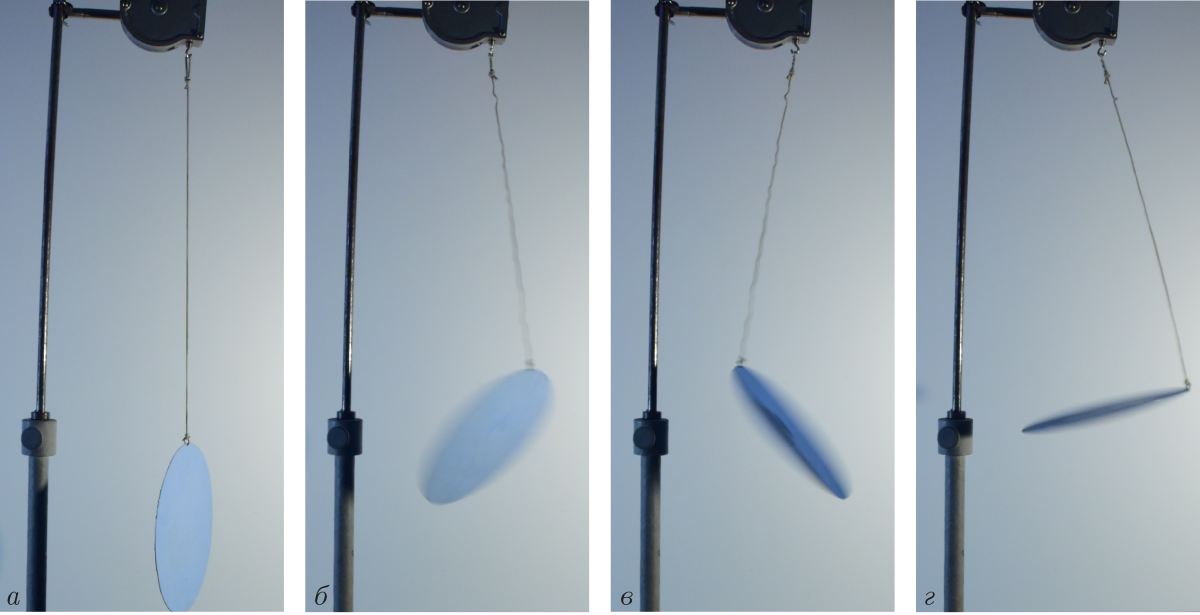
\includegraphics[width=0.9\linewidth]{freeaxis-3.png}
	\caption{Вращение алюминиевого диска вокруг главной оси инерции}
	\label{freeaxis-3}
\end{figure}

Одна из особенностей поведения тела при вращении проявляется в том, что центр масс тела поднимается в поле силы тяжести.

\begin{figure}[H]
	\centering 	
	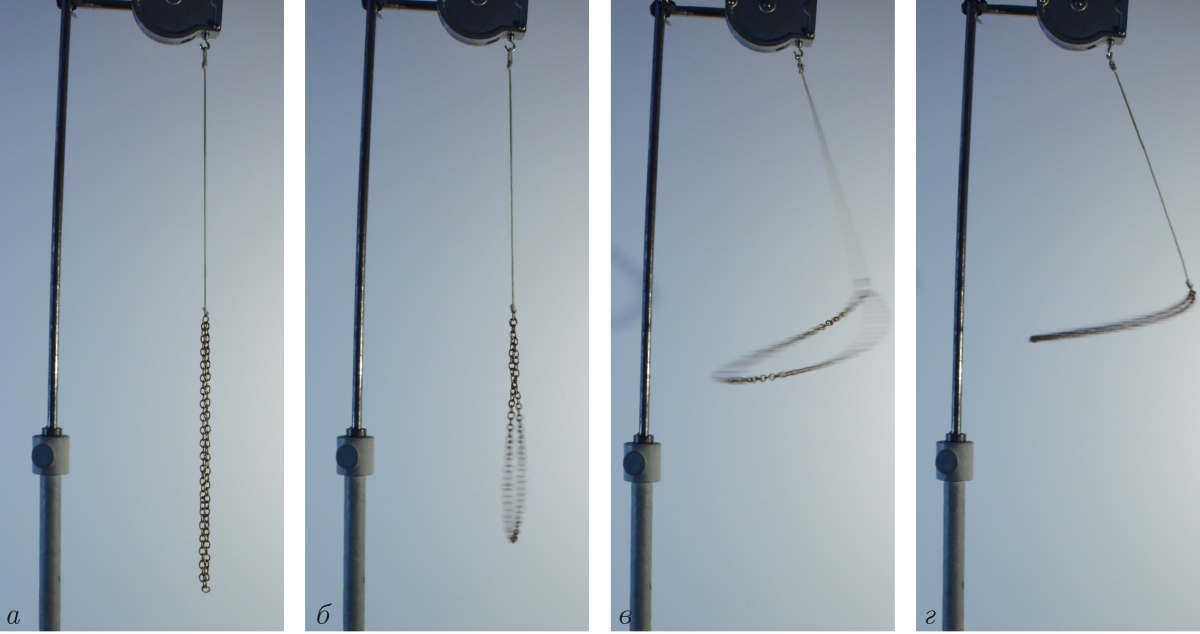
\includegraphics[width=0.9\linewidth]{freeaxis-4.png}
	\caption{Вращение металлической цепочки вокруг главной оси инерции}
	\label{freeaxis-4}
\end{figure}

\newpage
\subsection*{\underline{Теория:}}

Рассмотрим в качестве примера диск, вращающийся вокруг неподвижной вертикальной оси, которая смещена от центра диска на расстояние $ OC=b $ относительной неинерциальной системы отсчета. 
На тело действует сила тяжести \textit{m}\textbf{g}, и угловая скорость вращения равна \textbf{ω} (рис.\ref{freeaxis-5}).

Определим динамические реакции опоры в точках $ A $ и $ B $, если $ OA = OB = h $.
Будем предполагать что в точке $ A $ установлен подпятник, а в точке $ B $ — шарнир.

Проведем вращающиеся с диском оси $ Oxyz $ таким образом, чтобы ось $ y $ прошла через центр масс $ C $.
Ось $ Oz $ будет главной осью инерции диска для точки $ O $, поскольку плоскость $ Oxy $ является плоскостью симметрии диска.
Тогда момент инерции $ I_{xz} = I_{yz} = 0 $ и из условия $ \omega $ = const видно, что силы инерции приводятся к одной равнодействующей, проходящей через точку $ O $ и направленной вдоль линии вдоль оси $Oy$.
По модулю $$ F = ma_{c} = mb\omega^{2}. $$

\begin{figure}[H] 	
	\centering 		
	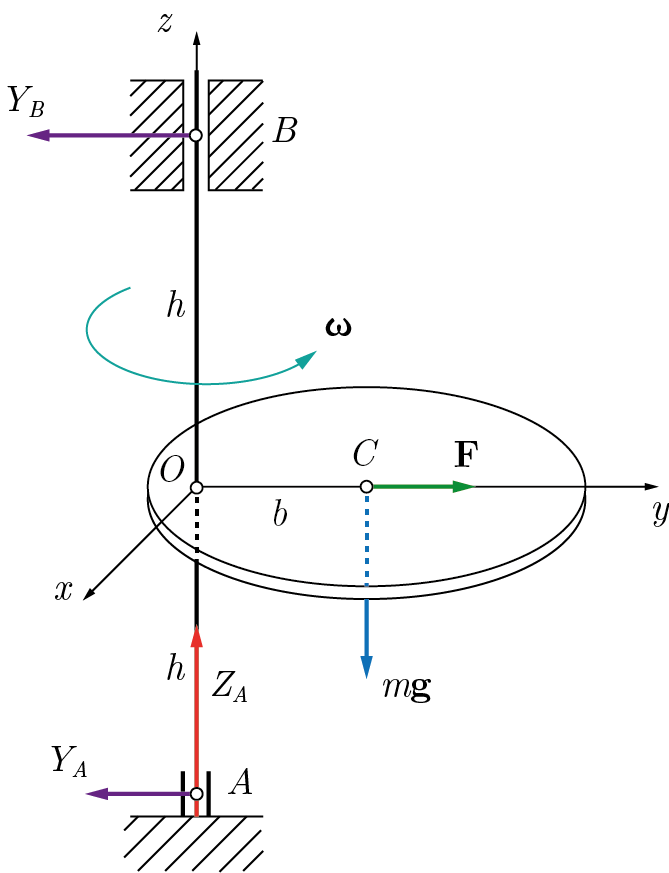
\includegraphics[width=0.5\linewidth]{freeaxis-5.png}
	\caption{При вращении твердого тела вокруг оси, концы которой жестко закреплены в подшипниках, возникающие в опорах динамические силы реакции уравновешиваются друг другом}
	\label{freeaxis-5}
\end{figure}

Так как векторы сил $ m\textbf{g} $ и $ \textbf{F} $ лежат в плоскости $ Oyz $, то реакции подшипников лежат в этой же плоскости, то есть имеют составляющие $ Y_{A} $ и $ Z_{A} $ в точке $ A $ и $ Y_{B} $ в точке $ B $. 
Тогда, составляя на основании принципа Даламбера для всех действующих сил и сил инерции уравнения равновесия в проекциях на оси $ Oy $ и $ Oz $ и уравнение моментов относительно центра $ A $, получим:

\begin{eqnarray}\label{freeaxis-eq1}
F -  Y_{A} -  Y_{B} = 0, \\
Z_{A} - mg = 0,\\
Y_{B}2h - mgb-Fh=0.
\end{eqnarray}

Решая эти уравнения, найдем:
\begin{eqnarray}\label{freeaxis-eq2}
Y_{B} = mgb\left(\frac{\omega^{2}}{2g} + \frac{1}{2}h\right), \\
Y_{A} = mgb\left(\frac{\omega^{2}}{2g} - \frac{1}{2}h\right),\\
Z_{A} = mg.
\end{eqnarray}

Таким образом, реакции $ Y_{A} $ и $ Y_{B} $ все время располагаются в плоскости $ Oyz $, вращающейся вместе с телом.

\end{document}
